% ================================ STORIA DI AES ======================================

\chapter{Storia di AES}

% ======================================================================================

%TODO: stream cipher vs block cipher \section
%TODO: kerchoffs laws \section.

% ---------------------------- SECTION: INTRODUZIONE ----------------------------------

%\newpage

\section{Introduzione}

%TODO: \textsf o \textsc o altro ?

%TODO: a blocchi simmetrico o a blocchi simmetrici?
\textsf{\small \textbf{AES} (\emph{\textbf{A}dvanced \textbf{E}ncryption \textbf{S}tandard}) è un cifrario a blocchi simmetrico, inventato da due matematici belghi, Vincent Rijmen e Joan Daemen, da cui viene il nome \emph{Rijndael}, nel 1998 per sostituire il precedente standard: DES (\emph{\textbf{D}ata \textbf{E}ncryption \textbf{S}tandard}).}

%TODO: aggiungere la differenza tra AES e Rijndael, sono diversi.
%TODO: Rijndael: gestisce blocchi e chiavi di differenti dimensioni. (blocco e chiave di 32 bit con 128 bit come minimo e 256 come massimo).
%TODO: AES: gestisce un blocco di dimensione fissa (128 bit) e la chiave può essere da 128, 192 o 256.

% ---------------------------- SECTION: STORIA DI AES ---------------------------------

%\newpage %TODO: questo newpage da problema, è da fixare

\section{Breve storia di AES} 

%TODO: Partire dal DES, dai problemi del DES e del triplo DES
%TODO: Nist 1997
%TODO: I concorrenti di AES: serpent, twofish, ecc. e dire per quale motivo è stato scelto Rijndael come AES alla fine.

\textsf{\small DES era divenuto lo standard dopo un bando dell'NBS (\emph{\textbf{N}ational \textbf{B}ureau of \textbf{S}tandards}), oggi NIST \emph{(\textbf{N}ational \textbf{I}nstitute for \textbf{S}ecurity and \textbf{T}echnology)} per trovare un buon e sicuro algoritmo per proteggere le comunicazioni private dei cittadini americani.}

%TODO: "rettificandone" o "alterandone"
\textsf{\small Venne così proposto un algoritmo chiamato \emph{Lucifer}, sviluppato dall'\emph{IBM} che dopo esser stato modificato dall'NSA (\emph{\textbf{N}ational \textbf{S}ecurity \textbf{A}gency}), riducendone la grandezza della chiave da 128 a 56 bits e rettificandone le funzioni contenute nell'S-box, venne designato come \emph{Data Encryption Standard} (\textbf{DES}).}

%TODO: "in lungo e in largo" magari è poco raffinata come espressione.
%TODO: questa è da rivedere! Mi sembra abbia poco senso compiuto
\textsf{\small DES regnò per 20 anni, venne studiato in lungo e in largo dagli accademici e criptoanalisti di tutto il mondo, grazie a ciò, ci fu finalmente per la prima volta un cifrario certificato che tutti potevano studiare: nacque così il moderno campo della crittografia.}

\textsf{\small Negli anni, molti sfidarono DES e dopo diverse battaglie fu finalmente sconfitto.} %TODO: ampliare come venne sconfitto?

%TODO: "fermare" o "ovviare"
%TODO: magari spiegare perché era lento più nel dettaglio. (perché combinevamo il des tre volte)
\textsf{\small L'unico modo per ovviare a questi attacchi era quello di combinare des tre volte, formando il 3DES (\emph{Triplo DES}). Il problema di questo però era la sua lentezza.} %TODO: estremamente lento


%TODO: "indire" è il verbo corretto?
\textsf{\small Per questo, nel 1997, il NIST indisse un nuovo bando per cercare un nuovo algoritmo di cifratura, forte come il triplo-DES, ma veloce e flessibile.}

\begin{figure}[H]
	\centering
	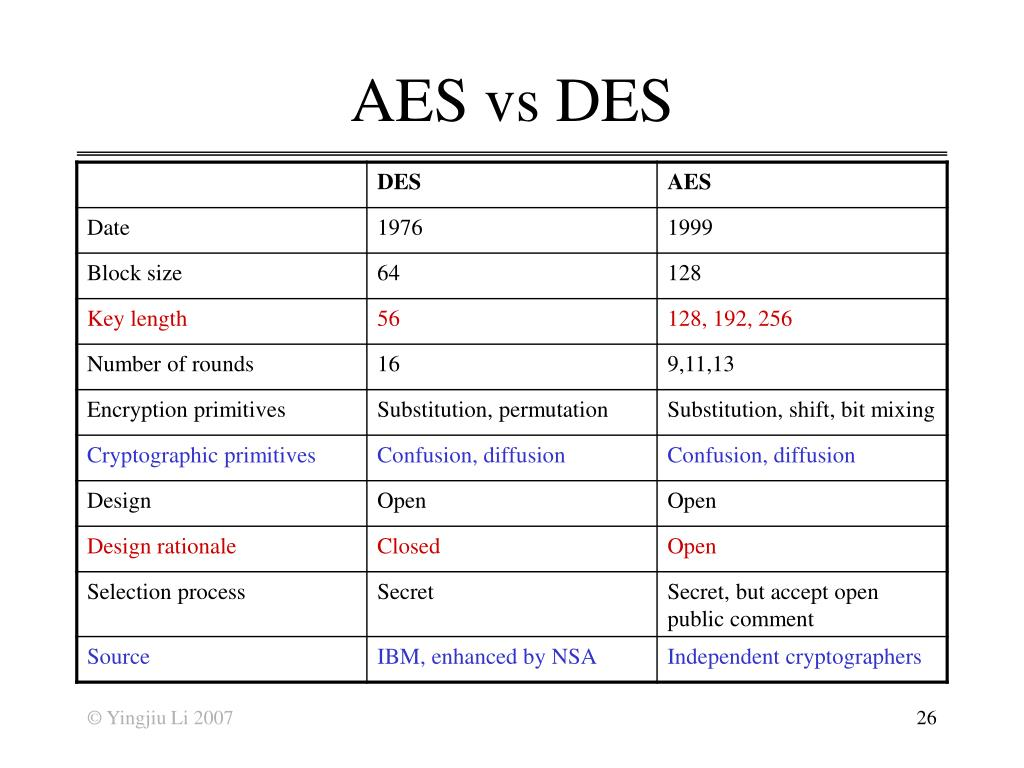
\includegraphics[width=1\textwidth, height=1\textheight, keepaspectratio]{./images/des_vs_aes/aes-vs-des.png}
	\caption{AES vs DES}
	\label{fig:aes_vs_des}
\end{figure}

%TODO: "spuntò" o "emerse" ?
%TODO: "semplicità"? Approfondire un po' di più magari
\textsf{\small Vari algoritmi competerono: Serpent, Twofish, MARS, RC6, ma alla fine spuntò Rijndael per la sua semplicità e velocità.} %TODO: magari aggiungere i link a pagine su questi algoritmi? con il footnote anche?

% ---------------------------- SECTION: AES VS RIJNDEAL ------------------------------

%\newpage

\section{AES vs Rijndeal}

\textsf{\small AES è un'implentazione di Rijndael, divenuto l'algoritmo di cifratura standard del governo degli Stati Uniti d'America.}
\textsf{\small Una differenza tra i due è che AES utilizza blocchi di dati da 128 bits, mentre Rijndael permette oltre a blocchi da 128, anche blocchi da 192 e 256 bits.} %TODO: "blocchi di dati"?

\textsf{\small Sia AES che Rijndael permettono una grandezza della chiave di 128, 192 o 256 bits, da cui ne ricaviamo il numero di rounds: 10, 12 o 14 rispettivamente.}

\begin{comment}
\begin{figure}[H]
	\centering
	\includegraphics[width=1\textwidth, height=1\textheight, keepaspectratio]{./images/.png}
	\caption{}
	\label{fig: }
\end{figure}
\end{comment}

%TODO: immagine AES vs Rijndael

% ------------------------ SECTION: SYMMETRIC VS ASYMMETRIC? --------------------------

%\newpage

\section{Cifratura simmetrica vs asimmetrica} %rinominare in "Cifrari simmetrici vs asimettrici"?

\textsf{\small Nella cifratura simmetrica viene usata una chiave sia per la cifratura che per la decifratura di un messaggio.}

\textsf{\small La cifratura asimmetrica è basata sul concetto di chiave pubblica e chiave privata. Vengono, quindi usate due chiavi sia per la cifratura che per la decifratura. Usiamo la chiave pubblica per cifrare il messagio e la chiave privata per decifrarlo.} %TODO: qui sto facendo un po' di controsenso.

\textsf{\small Ulteriori differenze: }

\begin{tabular}{|c|c|}
	\hline
	\textbf{Simmetrico} & \textbf{Asimmetrico} \\
	\hline
	\textsf{\small Richiede una sola  } & \textsf{\small Richiede due chiavi, } \\
	\textsf{\small chiave sia} & \textsf{\small  una pubblica e una privata,} \\
	\textsf{\small per la cifratura } & \textsf{\small una per cifrare e } \\
	\textsf{\small che la decifratura.} & \textsf{\small una per decifrare.} \\ %TODO: una per cifrare e una per decifrare?
	\hline
	\textsf{\small Lo spazio del testo cifrato è  } & \textsf{\small Lo spazio del testo cifrato è  } \\
	\textsf{\small lo stesso o più piccolo } & \textsf{\small lo stesso o più grande } \\
	\textsf{\small del messaggio originale.} & \textsf{\small del messaggio originale.} \\
	\hline
	\textsf{\small Il processo di cifratura } & \textsf{\small Il processo di cifratura } \\
	\textsf{\small è molto veloce.} & \textsf{\small è molto lento.} \\
	\hline
	\textsf{\small È usato quando un  } & \textsf{\small È usato per trasferire } \\
	\textsf{\small grosso ammontare di dati} & \textsf{\small piccole quantità} \\
	\textsf{\small deve essere trasferito.} & \textsf{\small  di dati.} \\
	\hline
	\textsf{\small Fornisce solamente } & \textsf{\small Fornisce confidenzialità, } \\ %TODO: non ripudio
	\textsf{\small la confidenzialità.} & \textsf{\small autenticità e non ripudio.} \\ %TODO: approfondire non ripudio?
	\hline
	\textsf{\small La chiave usata è di solito } & \textsf{\small La lunghezza della chiave } \\
	\textsf{\small di lunghezza 128 o 256 bits.} & \textsf{\small è di 2048 o più bits.} \\
	\hline
	\textsf{\small L'utilizzo delle risorse è basso.} & \textsf{\small L'utilizzo di risorse è alto.} \\
	\hline
	\textsf{\small Esempi: DES, 3DES, } & \textsf{\small Esempi: DSA, RSA, } \\
	\textsf{\small AES, RC4} & \textsf{\small Diffie-Hellman, ECC, El Gamal} \\
	%\textsf{\small } & \textsf{\small } \\
	\hline
\end{tabular}

\begin{figure}[H]
	\centering
	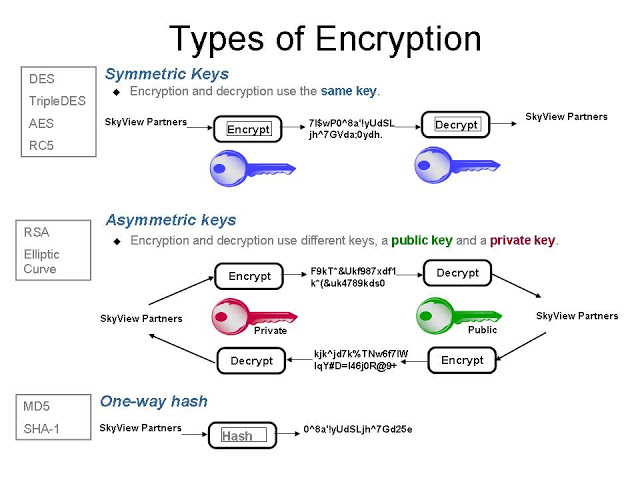
\includegraphics[width=1\textwidth, height=1\textheight, keepaspectratio]{./images/types_of_encryptions/types_of_encryption.png}
	\caption{Tipi di cifratura}
	\label{fig:encryption_types}
\end{figure}

\textsf{\small AES è di tipo simmetrico, quindi useremo la stessa chiave sia per cifrare il nostro messaggio sia per decifrarlo. }

\begin{figure}[H]
	\centering
	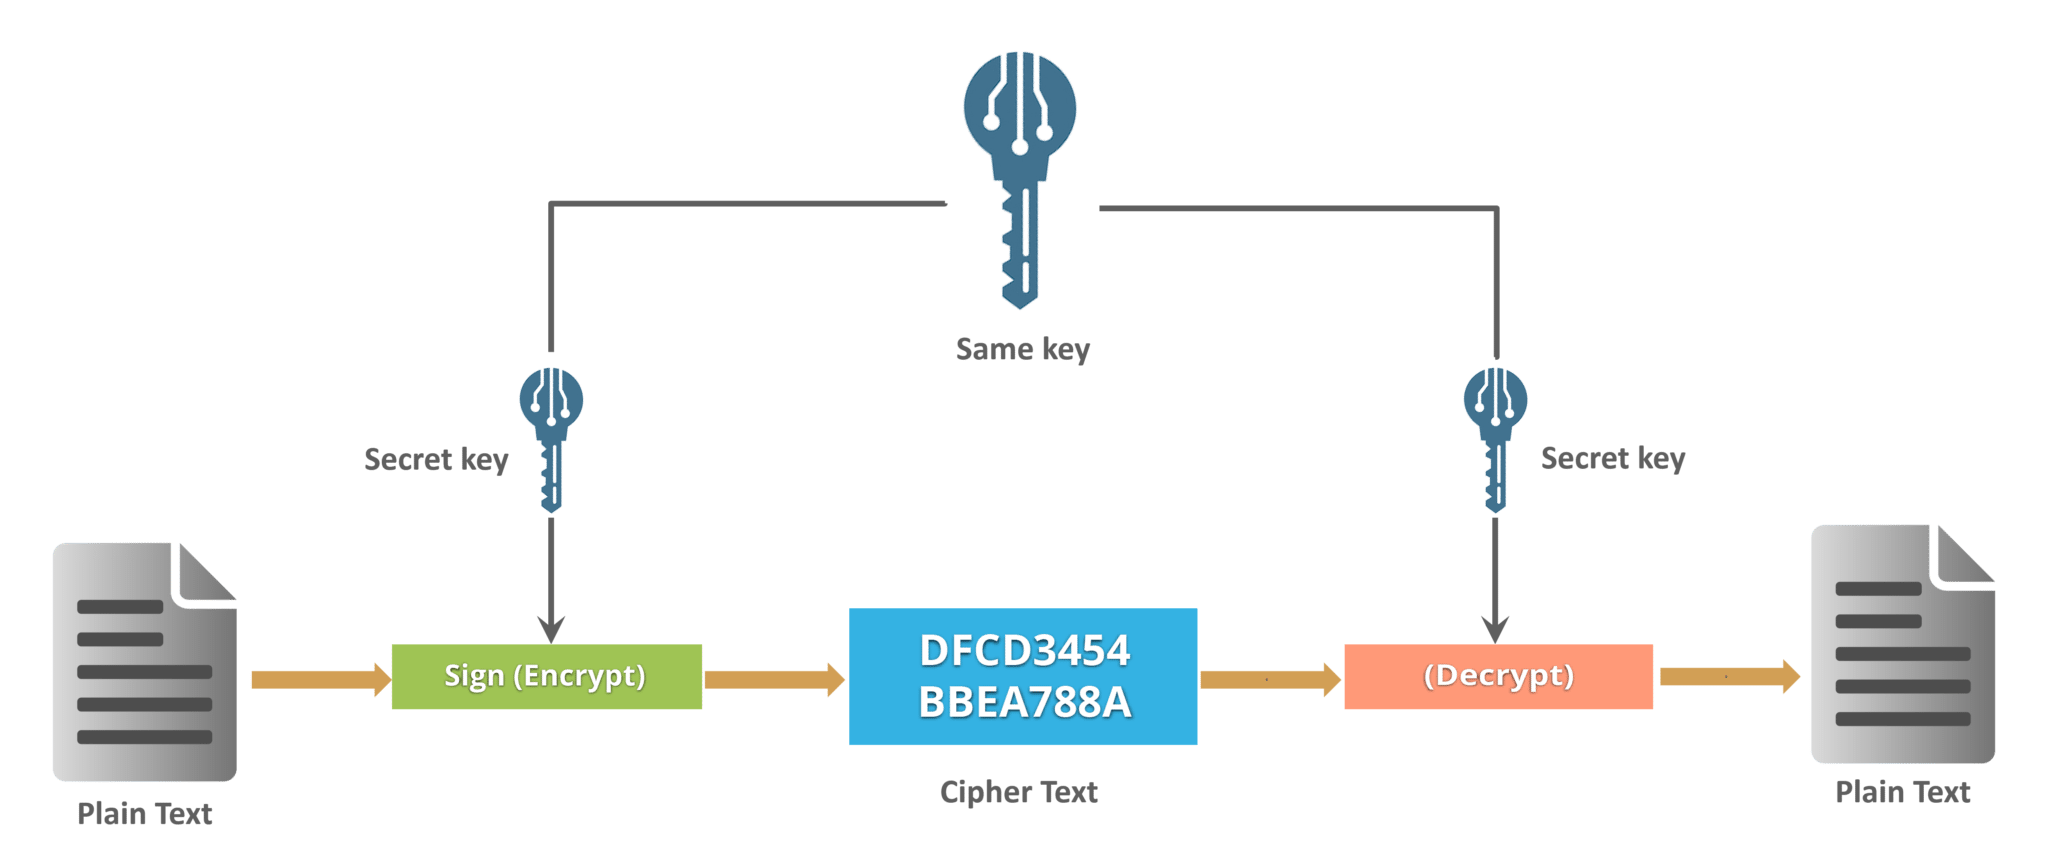
\includegraphics[width=1\textwidth, height=1\textheight, keepaspectratio]{./images/types_of_encryptions/symmetric_vs_asymmetric/symmetric-key-what-is-cryptography.png}
	\caption{Cifratura a chiave simmetrica}
	\label{fig:symmetric_encryption}
\end{figure}

% ------------------------ SECTION: STREAM VS BLOCK CIPHER ----------------------------

\section{Stream vs Block Ciphers}

\textsf{\small \textbf{Cifrario a flusso}: Il testo in chiaro viene separato in [singoli] bits che vengono poi singolarmente cifrati.} %TODO:

\textsf{\small \textbf{Cifrario a blocchi}: Un cifrario a blocchi prende un messaggio in chiaro e lo suddivide in blocchi di bytes.} %TODO: 

\textsf{\small  AES è un cifrario a blocchi che prende un blocco di grandezza fissa di 16 bytes (o 4 words).}

%TODO: aggiungere immagine?

% ------------------------ SECTION: PRINCIPIO DI KERCKHOFFS ---------------------------

\section{Principio di Kerchoffs}

\textsf{\small L'olandese Auguste Kerckhoffs elaborò, nel 1883, due articoli riguardanti la crittografia. Nel primo enunciò sei principi, di cui il più famoso (il numero 2) sostiene che la sicurezza di un sistema crittografico non deve risiedere nella segretezza del suo algoritmo, ma soltanto nel mantenere la sua chiave segreta.} %TODO:  [scrisse/redisse/stilò/compose/elaborò] nel 1883 due articoli riguardanti la crittografia. Nel primo trattò [enunciò] sei principi, di cui il più famoso (il numero 2) sostiene che la sicurezza di un sistema crittografico non deve risiedere nella segretezza del suo algoritmo, ma soltanto dal mantenere la chiave segreta.

\textsf{\small I sei principi di Kerckhoffs:} %TODO: 

%TODO: citare fonte.
%TODO: \cite{} Wikipedia e video.

\begin{enumerate}
	\item \textsf{\small Il sistema deve essere praticamente, se non matematicamente, indecifrabile.} %TODO: 
	\item \textsf{\small Non dovrebbe richiedere segretezza e non dovrebbe essere un problema se cade nelle mani nemiche.} %TODO:  [del nemico]
	\item \textsf{\small Deve essere possibile comunicare e ricordare la chiave, senza utilizzare note scritte e i corrispondenti devono essere in grado di modificarla a piacimento.} %TODO: Deve essere possibile comunicare e ricordare la chiave, senza utilizzare note scritte e i corrispondenti devono essere in grado di modificarla a volere/a piacimento.
	\item \textsf{\small ve essere applicabile a comunicazioni attraverso il telegrafo.} %TODO: 
	\item \textsf{\small  Deve essere portabile, e non dovrebbe richiedere diverse persone per poterlo utilizzare.} %TODO:
	\item \textsf{\small Il sistema dovrebbe essere facile da usare e non dovrebbe essere stressante o richiedere ai propri operatori di seguire una lunga lista di procedure.} %TODO: utenti
\end{enumerate}

% -------------------------------- FINE CAPITOLO --------------------------------------